\chapter{The Forward Model}
\label{ch:formodel}

In this Chapter, we present the forward model to which we apply our entire methodology and conduct a singular value analysis for different measurement scenarios to understand the forward model and to determine a sensible way to measure ozone. We follow the Michelson interferometer for passive atmospheric sounding (MIPAS) handbook~\cite{mipas2000handbook} and simulate data according to an idealised cloud-free atmosphere in local thermodynamic equilibrium, assuming a measurement instrument with infinite spectral resolution and no pointing errors.
This is a simplified forward model, and we do not include any other instrument-specific details, such as sensor area or antenna response, as they are not available to us. 
\begin{figure}[ht!]
	\centering
	\input{LIMB.pdf_tex}
	\caption[Schematic of measurement and analysis geometry.]{Schematic of measurement and analysis geometry, not to scale.
		The stationary satellite, at a constant height $h_\text{sat}$ above Earth, takes $m$ measurements along its line-of-sight defined by the line $\Gamma_j$.
		Each measurement has a pointing angle $\phi_j$ and a tangent height $h_{\ell_j}$, $j=1,2,\dots,m$ defined as the closest distance of $\Gamma_j$ to the Earth's surface.
		Between $h_{L,0} \approx 7$km and $h_{L,n} \approx 83$km, the atmosphere is discretised into $n$ layers as illustrated by the solid green lines.}
	\label{fig:LIMB}
\end{figure}

\section{Radiative Transfer Equation}
A satellite at a constant height $h_{\text{sat}}$ points through the atmosphere (limb-sounding) and measures thermal radiation of gas molecules along its straight line of sight $\Gamma_j$, see  Figure~\ref{fig:LIMB}.
One measurement of the thermal radiation of one specific molecule, in our case ozone, denoted by the ozone volume mixing ratio (VMR) $x(r)$ at distance $r$ from the satellite, at the wave number $\nu$, is given by the path integral
\begin{align}
	\label{eq:RTE} 
	y_j =   \int_{\Gamma_j}  B(\nu,T) k(\nu, T)   \frac{p(T)}{k_{\text{B}} T(r)}  x(r)  \tau(r) \text{d}r + \eta_j \, \\
	\tau(r) = \exp{ \Bigl\{ - \int^{r}_{r_\text{obs}}  k(\nu, T)   \frac{p(T)}{k_B T(r^{\prime})}  x(r^{\prime}) \text{d}r^{\prime} \Bigr\} } \, ,\label{eq:absRTE} 
\end{align}
which is the radiative transfer equation (RTE)~\cite{mipas2000handbook}.
For more information on the processes within the atmosphere for ozone, we refer to~\cite{Lee2020NightOzone}.
We define a tangent height $h_{\ell_j}$ and $\Gamma_j$ for each $j=1,2,\ldots,m$, so that the data vector $\bm{y} \in \mathbb{R}^m$ including some additive noise $\eta_j$.
Additionally, the pointing angle $0 \leq \phi_j < \phi_{\text{max}}$ is defined so that if $\phi = 0 \text{arc sec}$ the satellite points at $h_{L,0}$ and for a pointing angle $\phi_{\text{max}}$ at $h_{L,n}$.
Within the atmosphere, the number density $p(T) / (k_{\text{B}} T(r))$ of molecules is dependent on the pressure $p(T)$, the temperature $T(r)$, and the Boltzmann constant $k_{\text{B}}$.
The factor $\tau(r)\leq 1$ accounts for re-absorption of the radiation along the line-of-sight, which makes the RTE non-linear.
The absorption constant
\begin{align}
	k(\nu, T) = L(\nu, T_{\text{ref}}) \frac{Q(T_{\text{ref}})}{Q(T)} \frac{ \exp{\{ - c_2 E^{\prime \prime} / T\}} }{\exp{\{ - c_2 E^{\prime \prime} / T_{\text{ref}} \}}} \frac{ 1- \exp{\{ - c_2 \nu  / T \}} }{1 - \exp{\{ - c_2 \nu / T_{\text{ref}} \}}}
\end{align}
is dependent on the line intensity $L(\nu, T_{\text{ref}})$ at reference temperature $T_{\text{ref}} =296K $, the lower-state energy $ E^{\prime \prime} $ in $\text{cm}^{-1}$ of the targeted transition and the second radiation constant $c_2\coloneqq hc/k_{\text{B}} \approx 1.44\text{cmK}$ as in the HITRAN database \cite{gordon2022hitran2020}, with Planck's constant $h$ and speed of light $c$.
Since we assume that the measurement device has a negligible frequency window, we neglect line broadening around $\nu$ for the calculations of $L(\nu, T_{\text{ref}})$, which would normally be modelled as a convolution of the normalised Lorentz profile (collisional/pressure broadening) and the normalised Doppler (thermal broadening) profile~\cite{mipas2000handbook}.
Additionally, we target one specific molecule and calculate $k(\nu, T)$ accordingly, which usually would involve summing the individual absorption constants for multiple radiating molecules weighted by their respective VMR~\cite{mipas2000handbook}.
The total internal partition function is given as:
\begin{align}
	Q(T )= g^{ \prime} \exp{\{ - \frac{ c_2 E^{ \prime} }{T}\}} + g^{\prime \prime} \exp{\{ - \frac{ c_2 E^{\prime \prime} }{T}\}} \, ,
\end{align}
with the statistical weight $ g^{\prime \prime}$ for the lower and $ g^{ \prime}$ for the upper energy state (also called the degeneracy factors) accounting for the molecule's non-rotational and rotational energy states (see~\cite{vsimevckova2006einstein}), and the upper state energy $E^{ \prime} = E^{ \prime\prime} + \nu$.
Under the assumption of local thermodynamic equilibrium (LTE), the black body radiation acts as a source function
\begin{align}
	B(\nu,T)   = \frac{2 h c^2 \nu^3}{\exp{\{\frac{c_2\nu}{ T}\}}-1}\, .
\end{align}

For fundamentals on the RTE, we recommend~\cite[Chapter 1]{rybicki2000rte}, and for a more comprehensive model, we refer to \cite{read2006forwardModel}.



\section{Simulate Data Based on a Ground Truth}
\label{sec:SimDat}
To calculate the integrals in Eq.~\ref{eq:RTE} and Eq.~\ref{eq:absRTE} numerically, we discretise the atmosphere in $n$ layers and define height values $h_{L,i-1} < h_{L,i}$ with respect to the surface of the earth, for $i = 1, \dots, n$.
The $i$-th layer is defined by two spheres around the centre of the earth with radii $ r_0 + h_{L,i-1} $ and $r_0 + h_{L,i}$.
Then the ozone VMR $\bm{x} =\{x_1,x_2,\ldots,x_n\} \in \mathbb{R}^{n}$, pressure $\bm{p} =\{p_1,p_2,\ldots,p_n\} \in \mathbb{R}^{n}$ and temperature $\bm{T} =\{T_1,T_2,\ldots,T_n\} \in \mathbb{R}^{n}$, as well as all other height dependent parameters, are discretised profiles with constant values between the heights $h_{L,i-1} \leq h < h_{L,i}$.
Above $h_{L, n}$ and below $h_{L,0} $, the ozone VMR is set to zero, so no signal can be obtained.
We evaluate the integral in Eq.~\eqref{eq:RTE} for one noise-free measurement $A_{j}(\bm{p},\bm{T},\bm{x})$, using the trapezoidal rule.
Here, each entry $A_{j}$ of $\bm{A}(\bm{p},\bm{T},\bm{x})\in \mathbb{R}^{m}$ includes multiple evaluations of the integral in Eq.~\ref{eq:absRTE} to calculate the absorption $\tau(r)$.
%Note that, since we aim to provide estimates over pressure $\bm{p}$ and temperature $\bm{T}$, we explicitly include them as parameters in our forward model.
The data vector
\begin{align}
	\bm{y} = \bm{A}(\bm{x}) + \bm{\eta}\, 
\end{align}
includes an additive noise vector $\bm{\eta} \in \mathbb{R}^{m}$, where we define the non-linear forward model as $\bm{A}(\bm{x}) \coloneqq \bm{A}(\bm{x},  \bm{p},\bm{T})   \in \mathbb{R}^{m}$ for brevity.
Similarly, we define $\bm{A}_L\in \mathbb{R}^{m\times n}$, which denotes the linear forward model matrix and neglects absorption (e.g. set $\tau = 1$ in Eq.~\eqref{eq:absRTE}) and enables matrix-vector multiplication $\bm{A}_L \bm{x}$ to compute noise-free linear data.
Further, we classify the inverse problem as a weakly non-linear inverse problem, because neglecting the absorption changes the measurements only slightly (about $1\%$, see Chapter~\ref{ch:affine}).

As the ground truth for our methodology, we consider an ozone profile at distinct pressure values generated from some data~\cite{MLSdata} of the MLS on the Aura satellite within the Antarctic region.
This ozone profile has a peak in the middle atmosphere and a second peak at higher altitudes, see Fig.~\ref{fig:O3Samp}, which seems to be a typical nighttime profile~\cite{Lee2020NightOzone}.

We recursively relate pressure $p$ to geometric height $h$ with the hydrostatic equilibrium equation
\begin{align}
	\frac{\text{d}p}{p} = \frac{- g M}{R^* T} \text{d} h \, ,\label{eq:hydr}
\end{align}
starting with a pressure of $1013.25$hPa at sea level.
The acceleration due to gravity is
\begin{align}
	g = g_0 \Bigg( \frac{r_0}{r_0 + h} \Bigg) \, ,
\end{align}
where the polar radius of the earth is $r_0 \approx 6356 \, \text{km}$, the gravitation at sea level is $g_0 \approx 9.81 \text{m}/\text{s}^2$, $R^* = 8.31432 \times 10^{-3} \text{Nm} / \text{kmol} / \text{K}$ and the mean molecular weight of the air is $M = 28.97 \text{kg/kmol}$~\cite{atmosphere1976us}.
This holds up to a geometric height of $86$km, where we ignore a $0.04\%$ non-linear change in $M$ from $80$km to $86$km.

Following \cite{atmosphere1976us} we form the temperature function
\begin{equation}
	\label{eq:tempFunc}
	T(h) = \adjustbox{max width=0.825\textwidth}{$\begin{dcases*}
			T_0 &, \text{$h  = 0$}\\
			T_0 + a_0 h   &, \text{$0 \leq h < h_{T,1}$}\\
			T_0 + a_0 h_{T,1} &, \text{$h_{T,1} \leq  h < h_{T,2}$}\\
			T_0 + a_0 h_{T,1} + a_1 (h_{T,2}   - h_{T,1})  + a_2 (h   - h_{T,2})  &, \text{$h_{T,2} \leq h < h_{T,3}$}\\
			T_0 + a_0 h_{T,1} + a_1 (h_{T,2}   - h_{T,1})   & \\
			\hphantom{{} T_0 } + a_2 (h_{T,3}   - h_{T,2}) + a_3 (h   - h_{T,3}) &, \text{$h_{T,3} \leq h < h_{T,4}$}\\
			T_0 + a_0 h_{T,1} + a_1 (h_{T,2}   - h_{T,1})  & \\
			\hphantom{{} T_0 }+ a_2 (h_{T,3}   - h_{T,2})  + a_3 (h_{T,4}   - h_{T,3}) + a_4 (h   - h_{T,4}) &, \text{$h_{T,4} \leq h < h_{T,5}$}\\
			T_0 + a_0 h_{T,1} + a_1 (h_{T,2}   - h_{T,1})   & \\
			\hphantom{{} T_0 } + a_2 (h_{T,3}   - h_{T,2}) + a_3 (h_{T,4}   - h_{T,3}) + a_4 (h_{T,5}   - h_{T,4})& \\
			\hphantom{{} T_0 }  + a_5 (h   - h_{T,5}) &, \text{$h_{T,5} \leq h < h_{T,6}$}\\
			T_0 + a_0 h_{T,1} + a_1 (h_{T,2}   - h_{T,1})    &\\
			\hphantom{{} T_0}  + a_2 (h_{T,3}   - h_{T,2}) + a_3 (h_{T,4}   - h_{T,3}) + a_4 (h_{T,5}   - h_{T,4}) &\\ 
			\hphantom{{} T_0} + a_5 (h_{T,6}   - h_{T,5}) + a_6 (h   - h_{T,6})   &, \text{$h_{T,6} \leq h \lesssim  86$}
		\end{dcases*}$}\\
\end{equation}
with gradient and height values provided by~\cite{atmosphere1976us} (see Tab.~\ref{tab:tempGrad}) which acts as the ground truth temperature profile (see Fig.~\ref{fig:PriorTemp}).
\begin{table}
	\centering
	\begin{tabular}{ |c||c|c|  }
		\hline
		subscript $i$ & geometric height $h_{T,i}$ in km&gradient $a_i$\\
		\hhline{|=||=|=|}
		0& 0 & -6.5\\
		1& 11 & 0\\
		2& 20.1& 1\\
		3& 32.2& 2.8\\
		4& 47.4& 0\\
		5& 51.4& -2.8\\
		6& 71.8& -2\\
		\hline
	\end{tabular}
	\caption[Height depending temperature gradients]{Definition of height depending temperature gradients.}
	\label{tab:tempGrad}
\end{table}



We calculate one measurement according to the RTE as in Eq.~\ref{eq:RTE} and Eq.~\ref{eq:absRTE} using the trapezoidal integration rule.
We assume an atmosphere between $h_{L,1} = 6.9$km and $h_{L,n} = 83.3$km with $n = 45$ equidistant layers and a satellite at a fixed height of $h_{\text{sat}} = 500$km (see Fig.~\ref{fig:LIMB}).
The height value $h_{L,i}$ for each layer $i = 1,\dots, n$ is defined by the pressure values from~\cite{MLSdata} and the hydrostatic equilibrium equation, see Eq.~\ref{eq:hydr}.
We target ozone at a frequency of 235.71GHz, which lies within the region where the MLS observes ozone~\cite{livesey2008ozonecarbonmono, waters2006earth}.
The corresponding wave number is $\nu = 7.86\text{cm}^{-1}$.
We calculate the absorption constant $k(\nu,T)$ as in Eq.~\ref{eq:absRTE}, following the high resolution transmission (HITRAN) database~\cite{gordon2022hitran2020}, which provides the line intensity $L(\nu,T_{\text{ref}})$ for the isotopologue $\prescript{16}{}{\text{O}}_3$ with the AFGL Code 666.
%This gives us a non-linear forward model matrix $\bm{A}_{NL} = \bm{A}(\bm{x}, \bm{p}, \bm{T}) \in \mathbb{R}^{m \times n}$, where $\bm{x}\in \mathbb{R}^{n}$ is vector related to the ozone VMR, $\bm{p}\in \mathbb{R}^{n}$ is the vector describing the pressure values and $\bm{T}\in \mathbb{R}^{n}$ the temperature values.
Lastly, we add independent and identically-distributed Gaussian noise $\bm{\eta} \sim \mathcal{N}(0,\gamma^{-1} \bm{I})$ so that the $\text{SNR}=150$ (see Eq.~\ref{eq:SNR}) similar to~\cite{Froidevaux2008snrozone}, where a signal with a maximal spectral intensity of around $100\text{K}$ and a noise range of $0.4$ to $1.6\text{K}$ is reported.
We note that the methods used in this thesis will work with different SNRs or other frequencies.
Before computing a data vector $\bm{y} = \bm{A}(\bm{x}) + \bm{\eta} $ we decide for a measurement strategy with respect to the information provided by the forward model.

\subsection{Understanding the Forward Model}
%\textcolor{red}{understanding the forward map}
\label{sec:SVD}
By choosing a measurement strategy, we provide a quick and intuitive way of assessing if the data collection is effective, how much information is passed through the forward model, and how the signal-to-noise ratio (SNR) and the measurement strategy affect that information.
One way of doing this is via a singular value decomposition (SVD) of the linear forward model matrix $\bm{A}_L \in \mathbb{R}^{m \times n}$, which is given as
\begin{align}
	\bm{A}_L = \sum_{i =1}^{r} \bm{u}_i  \sigma_i \bm{v}^T_i = \bm{U} \bm{\Sigma} \bm{V}^T
\end{align}
with $r = \min\{m,n\}$.
Our main objective is to measure ozone $\bm{x}$, so our forward model $\bm{A}_L$ includes temperature and pressure, the latter is dominant, see Fig.~\ref{fig:PriorPressOverTemp}, decreases exponentially in height and hence does affect the information passed through the model.
If the pressure is high, the signal is large.
If the pressure is low, the signal is low, and the data tends to be noise-dominated.
%\textcolor{red}{The action of A on the paraemter
%Information about the projection of f along vk is “encoded” in the data as the component
%along the direction uk . The size of the projection is multiplied by sigma k to give the coefficient of
%uk , namely sigma k fk . The singular value is the factor which tells us by how much each component
%defining the image is amplified or attenuated when it is converted into the data
%not be changed in any way. If we now think of solving the inverse problem of reconstructing
%f from a measurement of d, it is clear that at best, those components of f along the first r
%right singular vectors are determined by the data. However the data tell us nothing at all
%about the components of f along the remaining n - r right singular vectors, and we have to
%use some other means for determining these components.}

The SVD of the forward model provides information on how $\bm{A}_L$, more specifically the right singular vectors $\bm{v}_i$, act on the parameter $\bm{x}$ since a noise-free measurement vector is given as $\bm{A}_L\bm{x}$.
The singular values $\sigma_i $, ordered in size from the largest $\sigma_1$ to the smallest $\sigma_{r}$, weigh that information from the right singular vectors to the left singular vectors $\bm{u}_i$.
Then the left singular vectors project $\sigma_i \bm{v}^T_i \bm{x} $ onto the data space.
For a large singular value, we can say that the forward model is informative about parameter structures according to the corresponding right singular vector. 
For a small singular value, we can say that the forward model is uninformative about parameter structures according to the corresponding right singular vector.
%\textcolor{red}{WQhat is the vice versa? Not clear what you are saying. }
%Note that we obtain the same results using the non-linear forward model $\bm{A}(\bm{x})$ to do this analysis, where we would rewrite to the matrix-vector multiplication $\bm{A}_{NL} \bm{x}$, where $\bm{A}_{NL}$ is depend on $\bm{x}$.
Further, if we define the SNR as
\begin{align}
	\text{SNR} \coloneqq \frac{\max(y)}{\text{STD noise}} = \frac{\text{peak signal}}{\text{RMS noise}} \label{eq:SNR} \, ,
\end{align}
we can roughly assume that the maximum singular value $\max(y) \approx \sigma_1$ and the information transmitted through the forward model corresponds roughly to the singular values $\sigma_i \gtrsim \max(y)/ \text{SNR}$ \cite{fox2025BlokkLecNot}.
Then, for very small singular values $\sigma_i \ll \sigma_1/\text{SNR}$ below the RMS noise level or the noise standard deviation (STD), an effective rank $r_{\text{eff}} \leq r$ is introduced.
The parameter space spanned by $ \{\bm{v}_{r_{\text{eff}} +1}, \dots ,\bm{v}_r \}$ is noise-dominated in the corresponding data space, see Figure \ref{fig:nullSpace}.
For singular values around the SNR, we expect reconstruction to have larger uncertainties, as that is where the noise is starting to influence the data.
For large singular values above the SNR, we expect reconstructions to be close to the ground truth as the corresponding data is hardly influenced by the noise.
See~\cite{tan2016LecNot} for a more comprehensive analysis.

\begin{figure}[ht!]
	\centering
	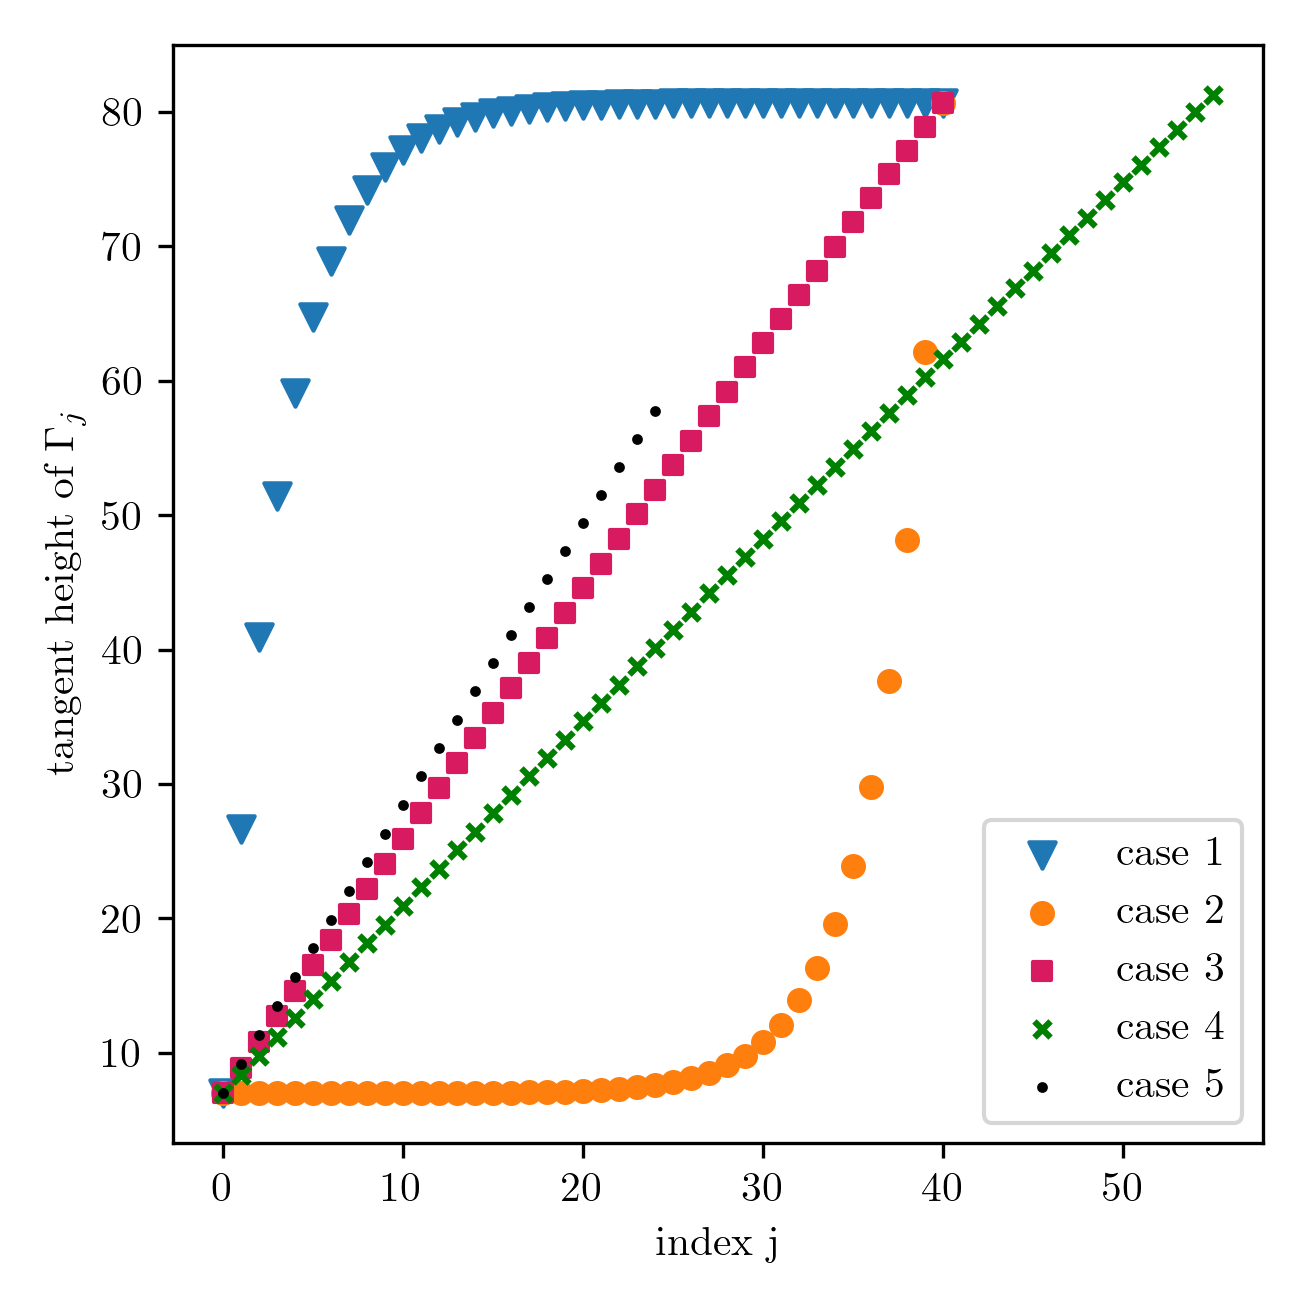
\includegraphics{MeasTangHeight.png}
	\caption[Tangent heights for different sequences of measurements.]{Tangent heights for five different sequences of measurements.}
	\label{fig:TangHCases}
\end{figure}
We test five different measurement strategies and plot the tangent heights corresponding to the pointing angles in Fig.~\ref{fig:TangHCases}.
The measurement test cases are:
\begin{itemize}
	\item \textbf{Case 1} includes 42 measurements between heights of $\approx7$km and $\approx83$km with pointing angles
	\begin{align*} 
		\phi_j  = \Bigg(\frac{-1}{1.25^{j-1}} + 1 \Bigg) \phi_{\text{max}} , \qquad  \text{for } j = 1, \dots, 42  \, .
	\end{align*}
	\item \textbf{Case 2} includes 42 measurements between heights of $\approx7$km and $\approx83$km with pointing angles
	\begin{align*} 
		\phi_j  = \frac{1.25 ^{j-1}}{ 1.25 ^{m-1}} 0.99 \phi_{\text{max}},  \qquad  \text{for } j = 1, \dots, 42\, .
	\end{align*}
	\item \textbf{Case 3} includes 42 measurements between heights of $\approx 7$km and $\approx 83$km with pointing accuracy $150 \text{arc sec}$ and pointing angles
	\begin{align*} 
		\phi_j  = (j-1) 150 \text{arc sec} ,  \qquad  \text{for } j = 1, \dots, 42\, .
	\end{align*}
	\item \textbf{Case 4} includes 83 measurements between heights of $\approx 7$km and $\approx83$km with pointing accuracy $77.5 \text{arc sec}$  and pointing angles
	\begin{align*} 
		\phi_j  =   (j-1) 77.5 \text{arc sec} ,  \qquad  \text{for } j = 1, \dots, 83\, .
	\end{align*}
	\item \textbf{Case 5} includes 30 measurements between heights of $\approx 7$km and $\approx 68$km with pointing accuracy $175  \text{arc sec}$ and pointing angles
	\begin{align*} 
		\phi_j  =  (j-1) 175 \text{arc sec} ,  \qquad  \text{for } j = 1, \dots, 30\, .
	\end{align*}
\end{itemize} 
Case 1 collects more data in low signal regions at high altitudes.
Case 2 collects more data in high signal regions at low altitudes.
Case 3, case 4, and case 5 measure at equidistantly spaced pointing angles corresponding to different pointing accuracies.
The pointing accuracy determines how well the satellite can point in a certain direction and, hence, the spacing of tangent heights in the atmosphere for a stable satellite at $h_{\text{sat}}$.
Case 1, case 2, case 3, and case 4 measure in between heights $h_{L,1} = 6.9$km and $h_{L,n} = 83.3$km, case 5 does not collect measurements in high altitude regions.
The pointing accuracy for case 3 in Fig.~\ref{fig:TangHCases} of $150\text{arc sec}$ was given to us by the team of the University of New South Wales Canberra Space~\cite{CubeSatInternal}.
Case 4 has half the pointing accuracy of case 3, and case 5 has a slightly larger pointing accuracy than case 3.
We visually assess the effective rank and how the singular values behave to determine which of the test cases is most effective.
More specifically, if the singular values decay fast and only a few singular values are above an SNR of 150, the forward map is rather uninformative.
If the singular values decay less fast and more singular values are above an SNR of 150, we classify the forward map as informative.
%\textcolor{red}{Another, they are multiplying like rabbits. Or flies. Which is more annoying?}
%\textcolor{red}{why is this plot here before you defined the cases? That's not remotely OK.}

\begin{figure}[ht!]
	\centering
	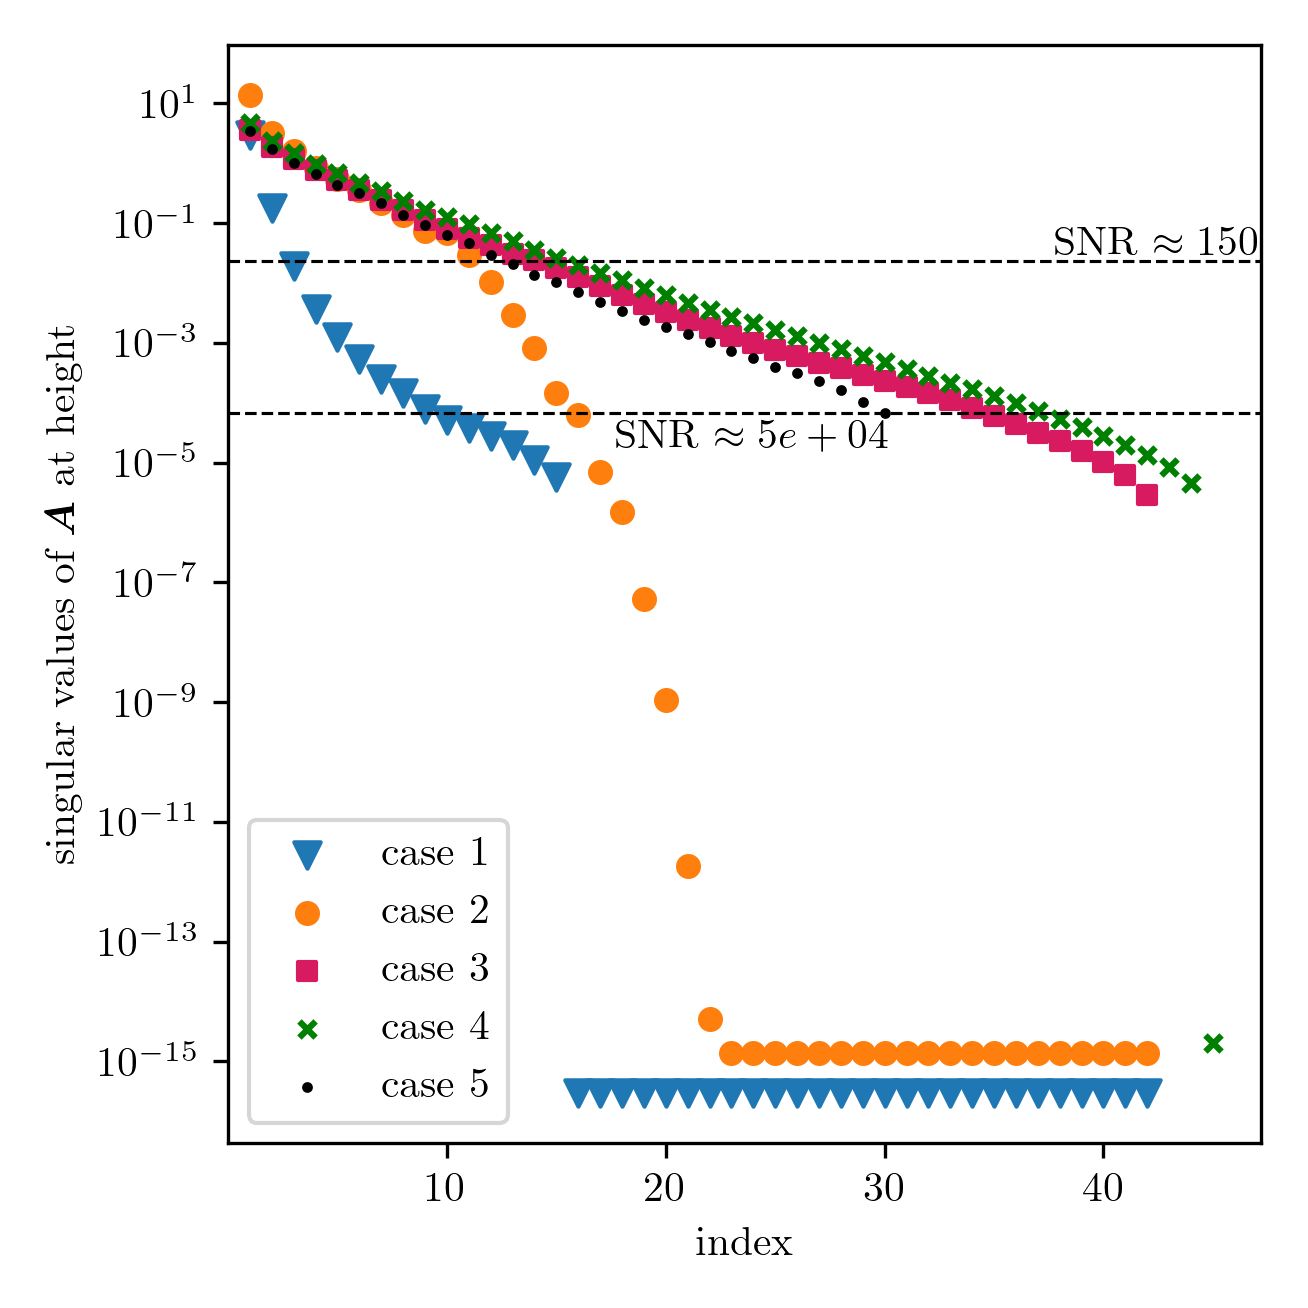
\includegraphics{SingValA.png}
	\caption[Singular values of linear forward model matrix for different sequences of measurements.]{Singular values of the forward model matrix for different sequences of measurements.
	The corresponding tangent heights of the test cases are plotted in Fig.~\ref{fig:TangHCases}. The dotted vertical line marks an SNR according to $\sigma_1$ of measurement case 5.}
\label{fig:SingA}
\end{figure}
In Fig.~\ref{fig:SingA}, we plot the singular values for each of the measurement cases.
The dotted lines in Fig.~\ref{fig:SingA} correspond to an SNR of roughly 150 with respect to the largest singular value of case 5 and an SNR according to the lowest singular value of case 5, which would be required to reconstruct all information provided by the forward model.
The largest singular value of case 5 has approximately the same value as the largest singular values of case 1, case 3, and case 4, so the SNR line is indicative for those cases as well.

Fig.~\ref{fig:SingA} shows that case 2 has the largest singular value of all cases, but its singular values decrease faster than the singular values of cases 3, 4, and 5 in the region where noise is becoming dominant.
In contrast, case 1 does obtain singular values which are decreasing the fastest of all cases and the largest number of singular values below an SNR of 150.
Additionally, cases 1 and 2 have a large number of very low singular values, and the smallest effective ranks of all cases, so we conclude that cases 1 nor 2 is effective.

The singular values of cases 3, 4, and 5 with equidistantly spaced pointing angles behave similarly and have larger effective ranks than case 1 or 2.
Case 4 measures almost twice as much compared to case 3, but does not provide much more information, which would justify the engineering effort required to achieve such pointing accuracy.
The slightly larger pointing accuracy in case 5 compared to case 3 provides similar information.
The last 5 to 10 singular values of case 3 are so small that the information will be completely covered by the noise.
Hence, we do not measure in noise-dominated regions and case 5 measures only up to a height of $\approx 68$km instead of $\approx83$km without losing too much crucial information above the SNR.
We note that if one wanted to obtain all information provided by the forward model, we would need an SNR of roughly $10^4$.
%\textcolor{red}{Oh come on, you are showing pictures of singular values without specifying exactly what the forward map and discretization is. That's not acceptable. If these are intended to be indicative, you need to be a damn site clearer about what they represent, and are trying to show.}
%\textcolor{red}{why? Explain your reasoning. If you don't say something specific, quantitative, it's just waffle.}
% \textcolor{red}{where is this spacing? At the satellite? A spacing in time? On the planet Mars. Be specific. All the way through, you need to tighten up loose statements like this.}
% 

%The corresponding singular values are plotted in Fig.~\ref{fig:SingA}, of which the first 25 decrease linearly in log-space and about 10-15 singular values lie above the SNR. \textcolor{red}{where is this spacing? At the satellite? A spacing in time? On the planet Mars. Be specific. All the way through, you need to tighten up loose statements like this.}
%In comparison, if we measure a lot of times in regions where the data is noise-dominated (high altitude), case 1, we do obtain more information since the singular values decrease rapidly.
%\textcolor{red}{Oh come on, you are showing pictures of singular values without specifying exactly what the forward map and discretisation are. That's not acceptable. If these are intended to be indicative, you need to be a damn site clearer about what they represent, and are trying to show.}
%Measuring lots of times at low altitudes, where the data is informative, and less at higher altitudes, case 2, does not seem optimal either, as we observe one larger singular value, but the other singular values decrease faster compared to case 3.
%Now consider case 4, where we double the number of measurements compared to case 3. We do get slightly larger singular values, but not so significantly that it would be worth the engineering effort required to achieve that.
%The measurements with equidistance-spaced tangent height seem to be most effective. \textcolor{red}{why? Explain your reasoning. If you don't say something specific, quantitative, it's just waffle.}
%By exploratory analysis, we find that we can tolerate a slightly larger distance between tangent heights (pointing accuracy of $175\text{arc sec}$) than required by~\cite{CubeSatInternal}, see case 5.
%In that case, we also stop measuring when the signal is too noisy and decrease the number of measurements taken without losing crucial information.
%We note that if one wanted to obtain all information provided by the forward model, we would need a signal-to-noise ratio of roughly $10^7$.

In principle, we show that it does matter how one measures, but one cannot get much more information by measuring more in regions where the information content is low or high.
The test cases show that an efficient measurement strategy may consist of equidistantly spaced pointing angles and does stop measuring when the singular values (information) are too low. 
Consequently, we proceed with case 5 and plot the right singular vectors of the forward model versus height in the atmosphere to see to which parameter structures our model is sensitive.
%\textcolor{red}{on the contrary - -you have just been arguing that it does matter. no, this makes sense if the goal is to reduce noise.}
%This contradicts the current measurement setup on the AURA MLS~\cite{livesey2006retrieval}, which reports high noise in lower atmospheric regions, due to thermal radiation from the earth, and measures more in those regions.

%\textcolor{red}{oh no, I had hpped this section would be 'we' free.}
%\textcolor{red}{where do you explain why this SNR has a line here?,
	%Were is the clear definition of these cases? I could not find it.}

\begin{figure}[ht!]
	\centering
	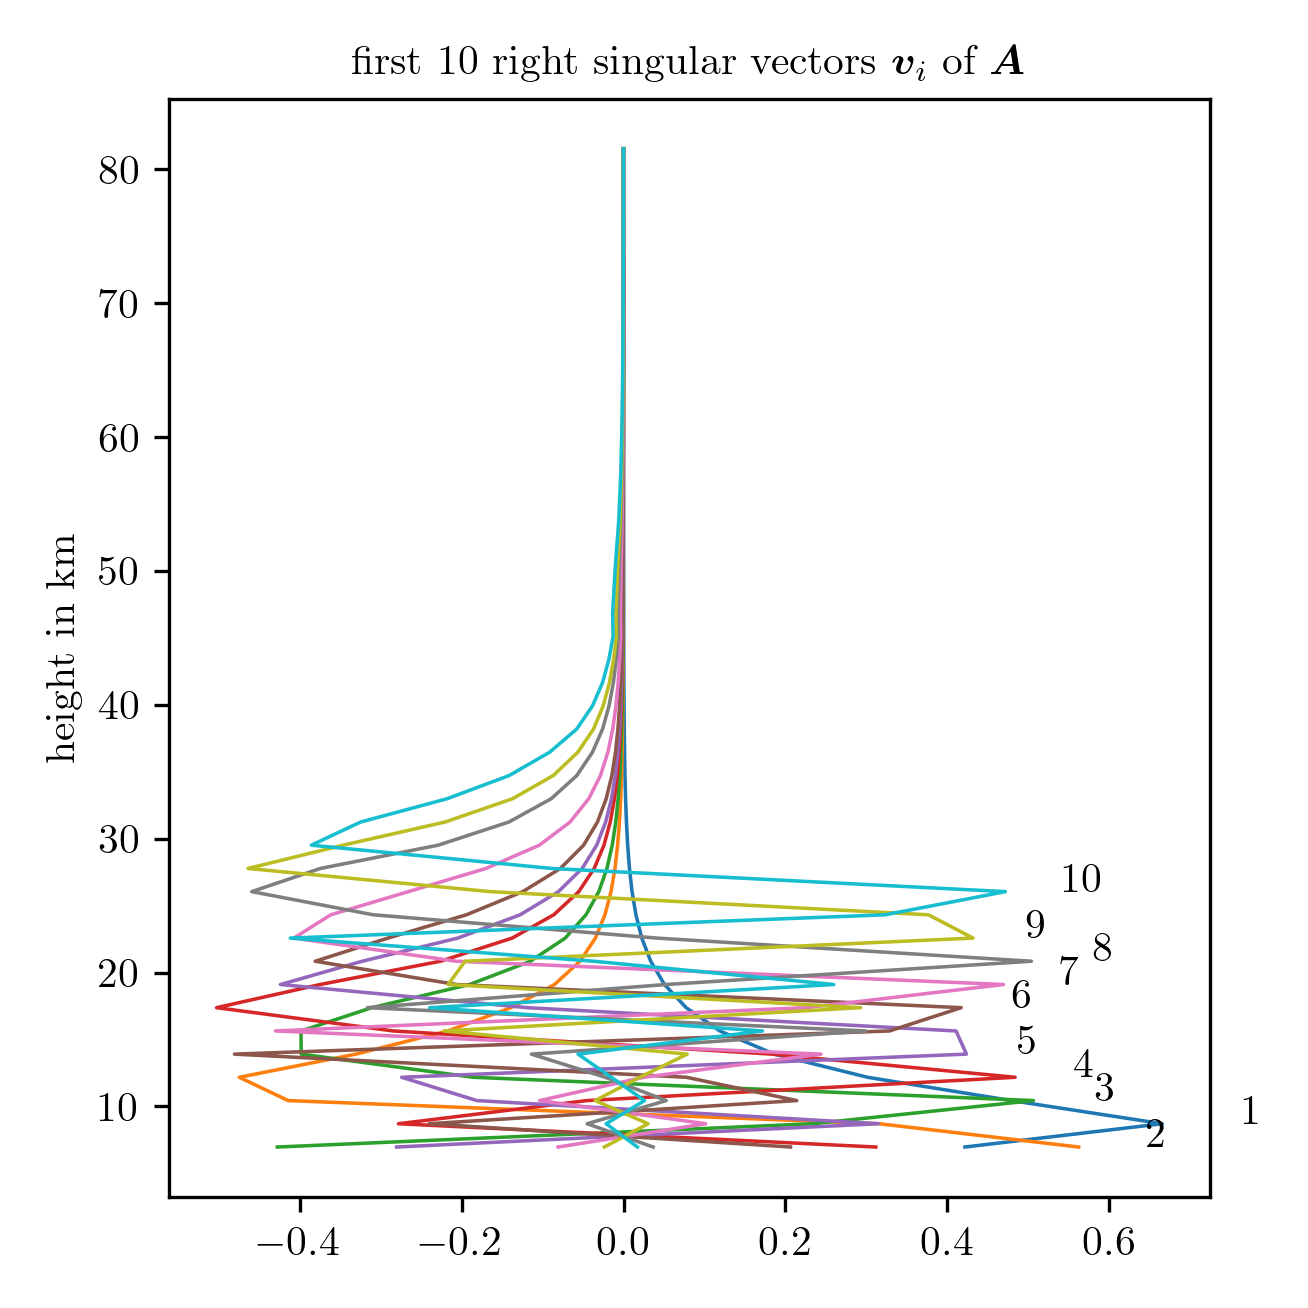
\includegraphics{SingVecA.png}
	\caption[First 10 right singular vectors of forward model.]{First 10 right singular vectors of the forward model matrix for measurements case 5 in Fig.~\ref{fig:TangHCases}. These singular vectors correspond to high singular values of the forward model in Fig.~\ref{fig:SingA}.}
	\label{fig:SingVecA}
\end{figure}
\begin{figure}[ht!]
	\centering
	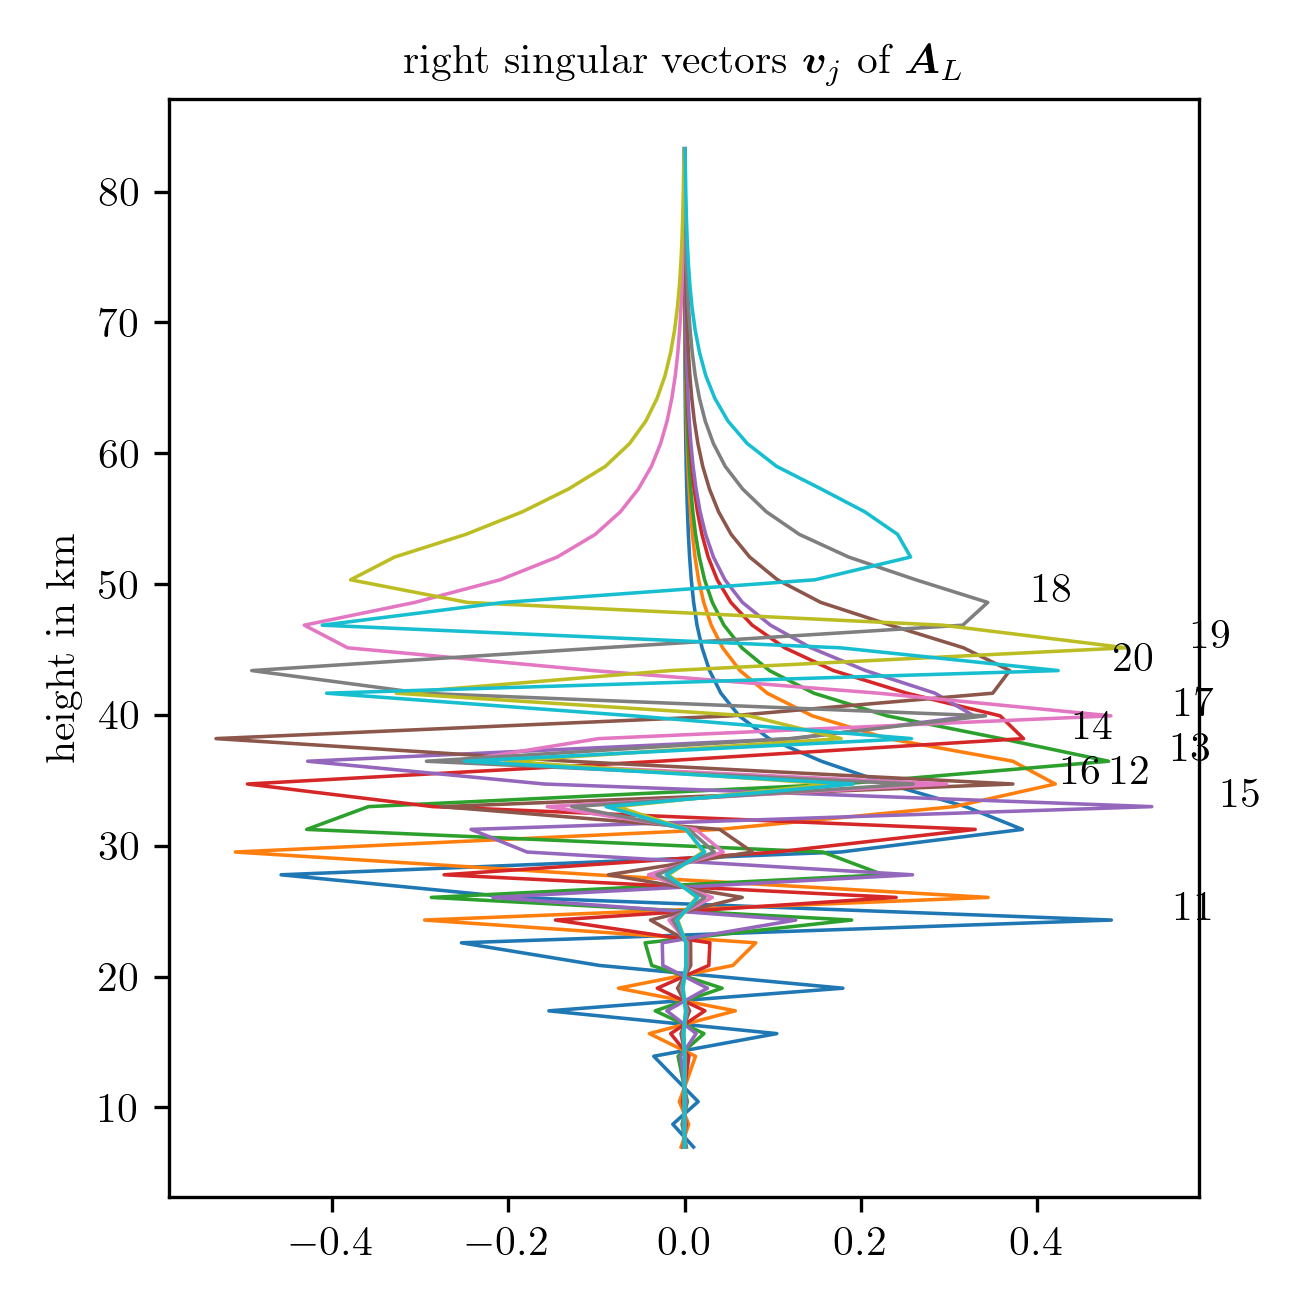
\includegraphics{MiddleVecA.png}
	\caption[Right singular vectors 11 to 19 of forward model.]{Right singular vectors with index $i = 11,\dots, 19$ of the forward model matrix for measurements case 5 in Fig.~\ref{fig:TangHCases}.
		These singular vectors correspond to singular values in Fig.~\ref{fig:SingA}, where the noise level is similar to the data.}
	\label{fig:middleSpace}
\end{figure}
\begin{figure}[ht!]
	\centering
	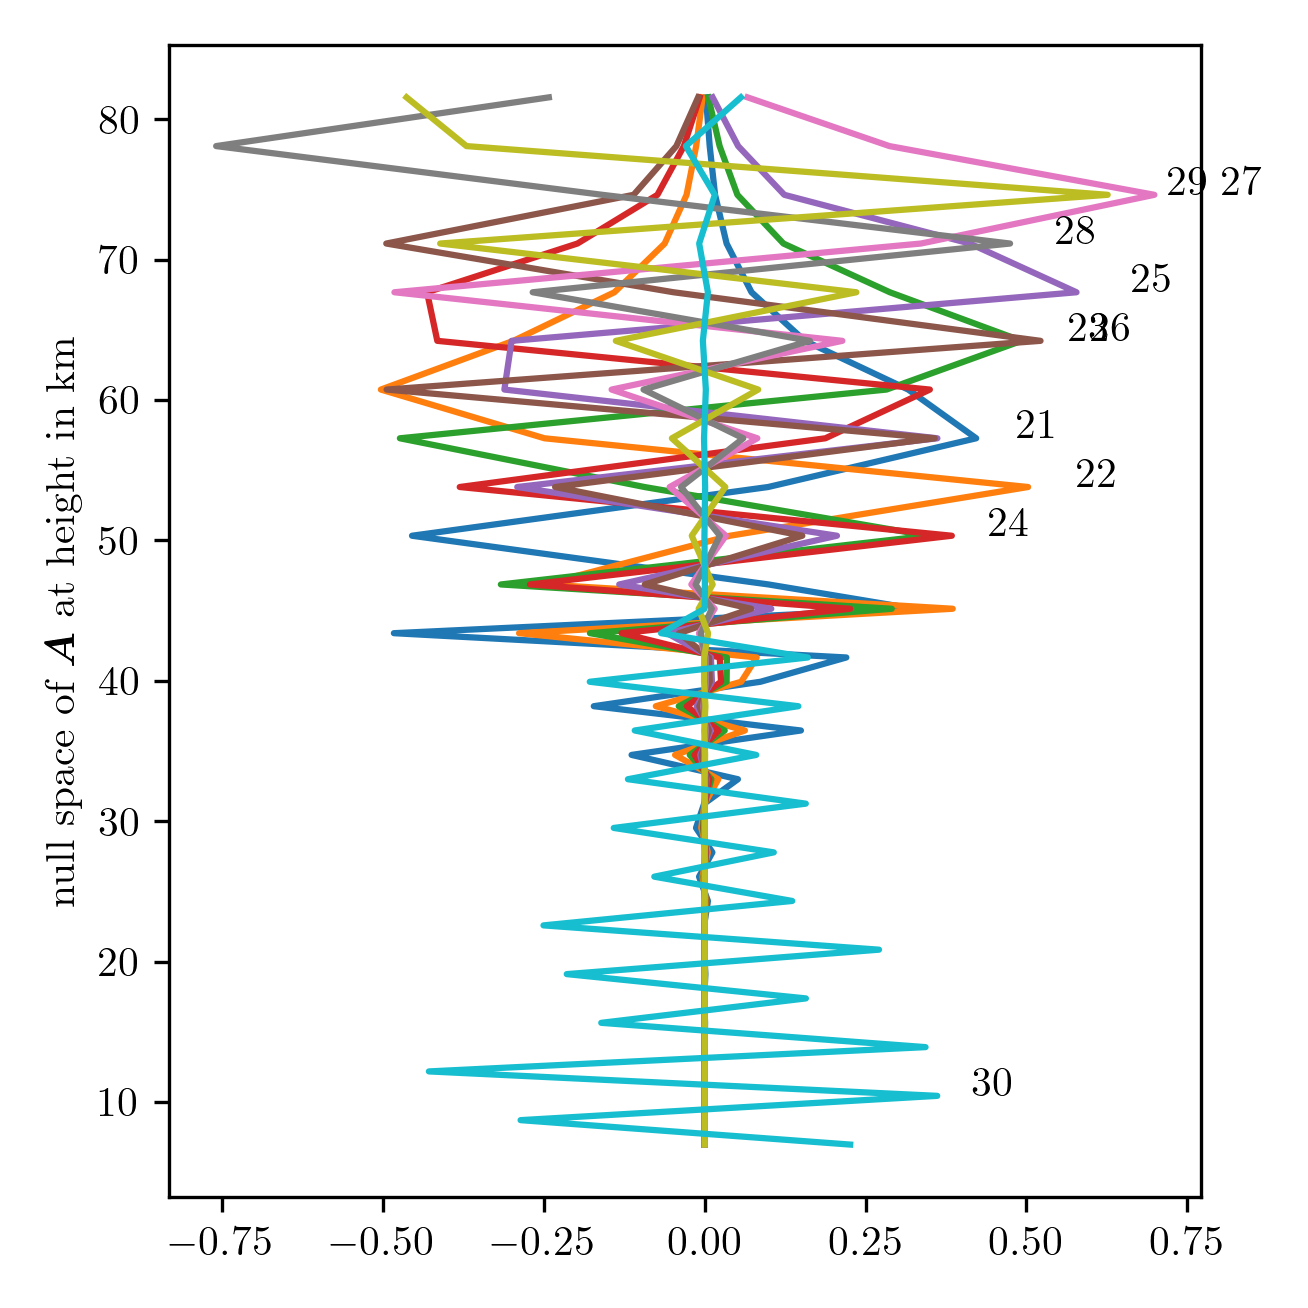
\includegraphics{NullVecA.png}
	\caption[Last 10 right singular vectors of forward model.]{Last 10 right singular vectors of the forward model matrix for measurements case 5 in Fig.~\ref{fig:TangHCases}. These singular vectors correspond to small singular values of the forward model in Fig.~\ref{fig:SingA}, where the data is noise-dominated.}
	\label{fig:nullSpace}
\end{figure}
The parameter space of $\bm{A}_L$ spanned by the first 10 right singular vectors plotted in Fig.~\ref{fig:SingVecA} corresponds to the 10 largest singular values in Fig.~\ref{fig:SingA} and represents parameter structures in the lower atmospheric regions.
So we can assume that, given some data, we will be able to provide good reconstructions of the parameter in lower altitudes up to $\approx30$km.
The right singular vectors in Fig.~\ref{fig:middleSpace} correspond to the singular values $\sigma_j$ for $j = 11, \dots, 20$ around the SNR of 150, in Fig.~\ref{fig:SingA}.
This is roughly where the noise starts to dominate the data, and the parameter space spanned by those right singular vectors represents parameter values in the middle atmosphere.
Consequently, we expect an increasing uncertainty of reconstructed parameter values at heights between $\approx20$km and $\approx55$km.
The singular vectors in Fig.~\ref{fig:nullSpace} corresponding to the smallest 10 singular values and span structures in parameter space at higher altitudes.
Since the singular values are very small, we will not be able to reconstruct parameter values from the ground truth above $\approx55$km and the data is noise-dominated.
More specifically, the retrieved parameter values at higher altitudes will be mostly determined by the prior or, in the case of regularisation, by the regulariser~\cite{tan2016LecNot}.

%The difference in between tangent heights is between 2.05km and 2.17km.
% \textcolor{red}{Actually, you should calculate this from the MIPAS specifications, or similar. It claims 1-3km resolution, presumably at a distance of 500km. So, what's that in arc seconds? It's also related to your vertical discretization, or, more to the point, your vertical discretization is determined by this.}
%  around the SNR,

\begin{figure}[th!]
	\centering
	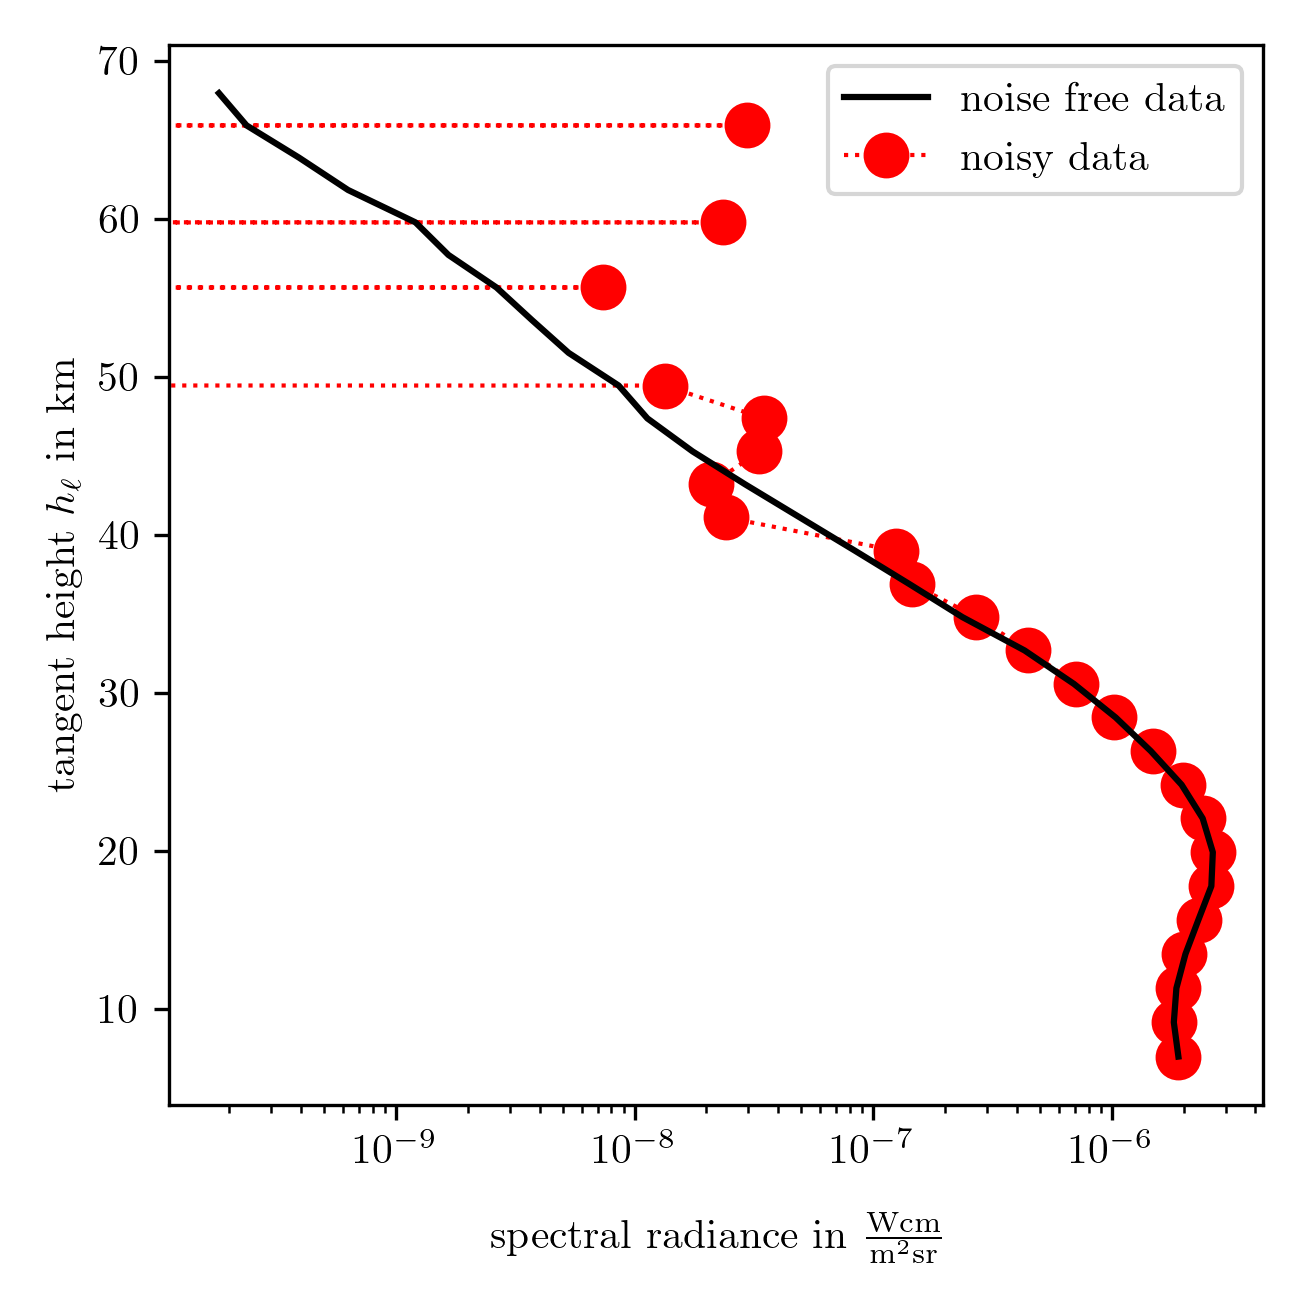
\includegraphics{DataPlot.png}
	\caption[Logarithmic plot of data points at different tangent height.]{Logarithmic plot of data points at different tangent height. Note that negative values are not plotted, and noise is dominating at higher altitudes.}
	\label{fig:DataPlot}
\end{figure}

Now we can compute a data vector $\bm{y} = \bm{A}(\bm{x}) + \bm{\eta} $, with $m = 30$ measurements determined by the satellite pointing accuracy of $175\text{arc sec}$ (see case 5 in Fig.~\ref{fig:TangHCases}), according to the RTE as in Eq.~\ref{eq:RTE} and Eq.~\ref{eq:absRTE} using the trapezoidal integration rule.
As already mentioned, we set the SNR to 150 and plot the data in Fig.~\ref{fig:DataPlot}, which is noise-dominated in higher altitudes.
Now, given the data, we like to determine the posterior distributions over ozone $\bm{x}$, pressure $\bm{p}$ and temperature $\bm{T}$.
\clearpage
